\chapter{ECG Raw Data}
The data used in this project is sourced from the Apnea-ECG dataset
 \cite{penzel2000apnea}, \cite{pollard_physionet_2026}. There are
 75 datasets each corresponding to the sleep of an individual, they contain
 an ECG signal with amplitude in millivolts, along with annotation files. Every dataset
 has a QRS annotation file that contain time annotations for the occurence of QRS Complexes, whilst 
 35 of the files contain a further annotation file indicating the presense of Apnea in minute increments
 \cite{penzel2000apnea}. The data is stored using WFDB conventions.\\

 Figure~\ref{fig:ecg-signal} encapsulates the form we want to convert the data and annotations into, i.e an array of waveform values
 and an associated time array, along with arrays that capture annotation value and time of occurence. 
\begin{figure}[H]
    \centering
    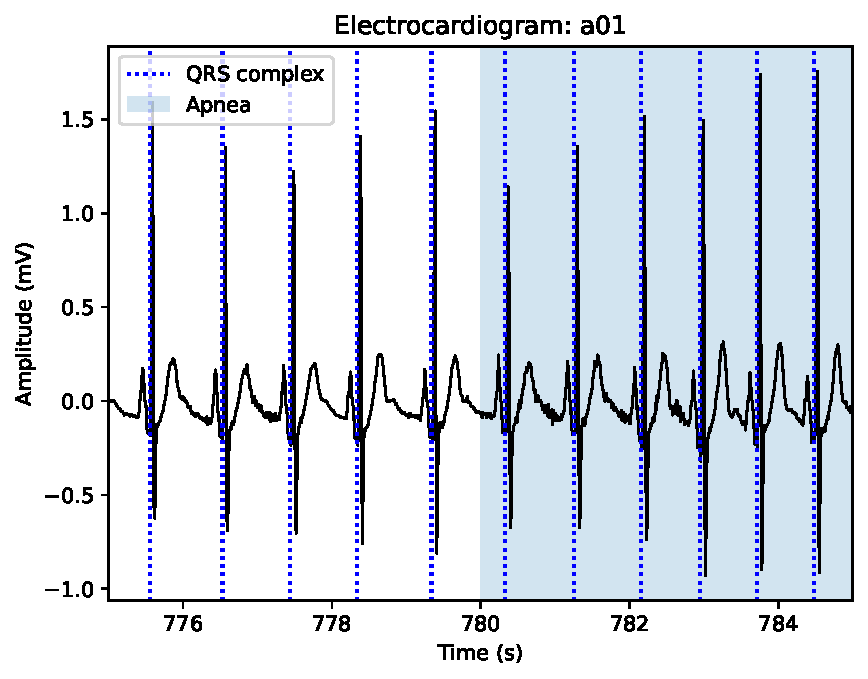
\includegraphics[width=0.50\textwidth]{figures/Example_ecg_signal.pdf}
    \caption{ECG signal along with QRS and Apnea Annotations.}
    \label{fig:ecg-signal}
\end{figure}

 \section{Data Processing}
To begin to analyse the ECG signal, we first need to understand how the data is stored. The data for the ECG 
waveform is stored in binary, and the way to parse the data is described 
by a header file that is written in ASCII. The description for how to read 
these header files is provided by \cite{physionet_wfdb}, under WFDB file formats (header). 
A header file contains two lines, the record line contains information that is relevant to all signals, 
for us the important information is regarding sampling frequency and number of signals, allowing us to extract our
timing information. The next step is to 
understand the signal, this is described by the signal line.  The key details are the format for which to extract the signal 
(this specifies how to convert binary into an integer data type), 
the specific formats are described by \cite{physionet_wfdb}, under WFDB file formats (signal). In the case of this project,
the data is stored in format 16, that is in 16 bits stored least significant byte first (i.e little endian) \cite{penzel2000apnea}, \cite{physionet_wfdb}.
This means the integer is given by arranging the bytes as second byte followed by first byte. 
Additionally, there is information about the ADC (anolog to digital conversion),
of relevance to this project is the ADC gain, dividing by this value will scale the integer data into
mV ready now for us to plot. \\

Extracting annotations requires a little more work, and the full description for how to go about this is
given by \cite{physionet_wfdb}, under WFDB file formats (annot). The overview is as follow, the data comes in a pair;
an A value and an I value, the A value corresponds to the annotation in our case normal or Apnea occurence and 
the I value whichs specifies how long after the previous annoation this annotation occured, for the first one that is time after the start 
for which it occured. 
The information for these two comes in 16 bits, the 6 most significant bits (in our case the last 6 as its implemented
least significant byte first) correspond to the annotation, and the first 10 bits correspond to the 
interval. There is one caveat, that is if the annotation gives the 
numerical value 59 (note there are other values but these are irrlevant to this projects data), 
this specifies a skip and needs to be handled differently, as it means the 
next 4 bytes of information tell you an extended time interval for which to add to the interval 
of the upcoming annotation (the next annotation takes longer to occur). The binary information of 
the next 4 bytes can be thought of as two chunks of bytes, the first being the high and the
last the low, each chunk read using the little endian method as we have done before. 
Then the interval is given by the integer associated with high chunk then low chunk. \\

Figure~\ref{fig:data_process} summarises how each data form is read. 
\begin{figure}[H]
    \centering
    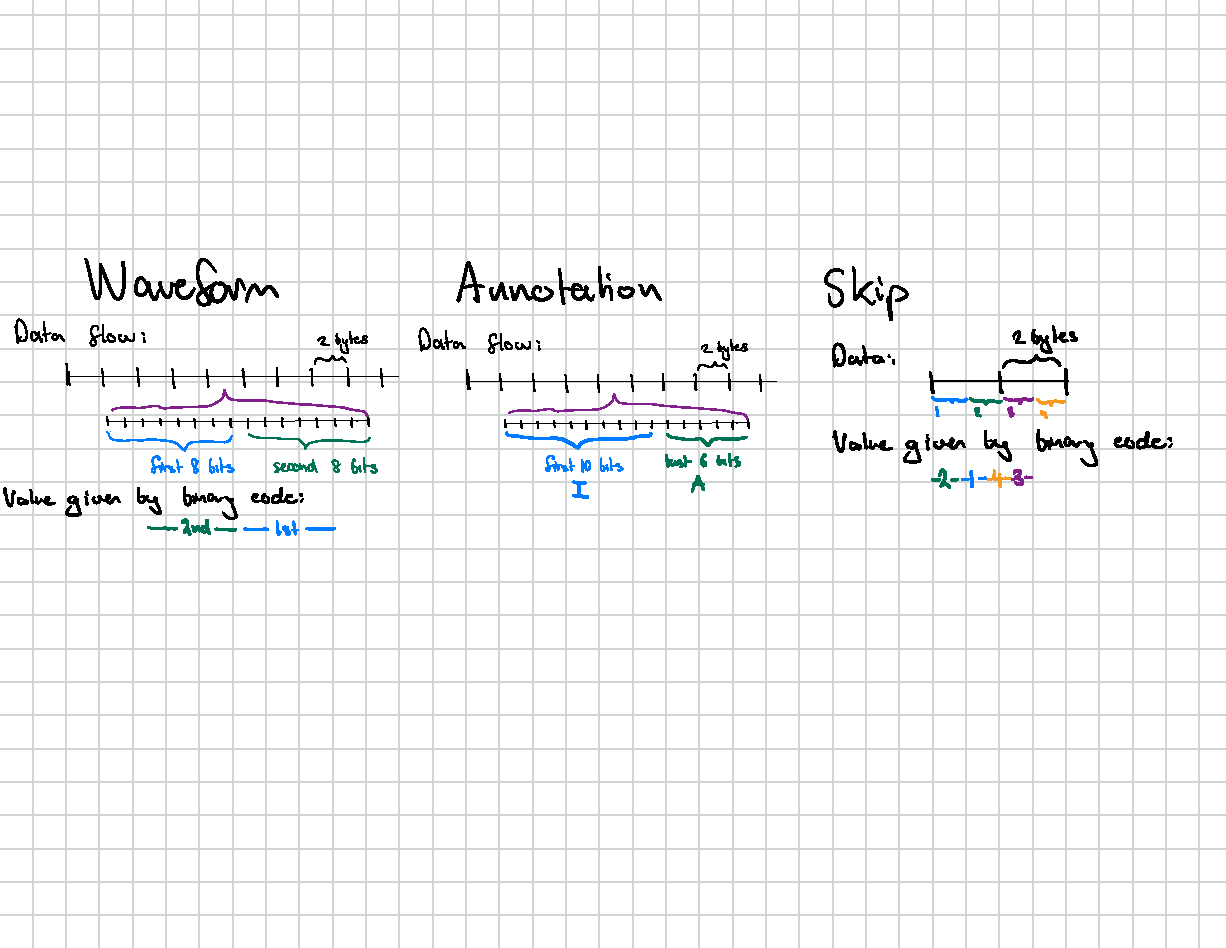
\includegraphics[width=\textwidth, trim={0cm 6cm 0cm 3.5cm},clip]{figures/data_process.pdf}
    \caption{Visual for how to process each data form.}
    \label{fig:data_process}
\end{figure}

\section{Preliminary Signal Exploration}
As we are working with ECG signals, the amplitudes and time intervals differ across time and samples due 
to morphological differences in humans, along with noise and artifacts picked up in the data collection 
process \cite{valerian2026respiratory}. We now illustrate a few samples that show these differences, these samples will give a basis
of data to check our algorithms for robustness. 
\begin{figure}[H]
    \centering
    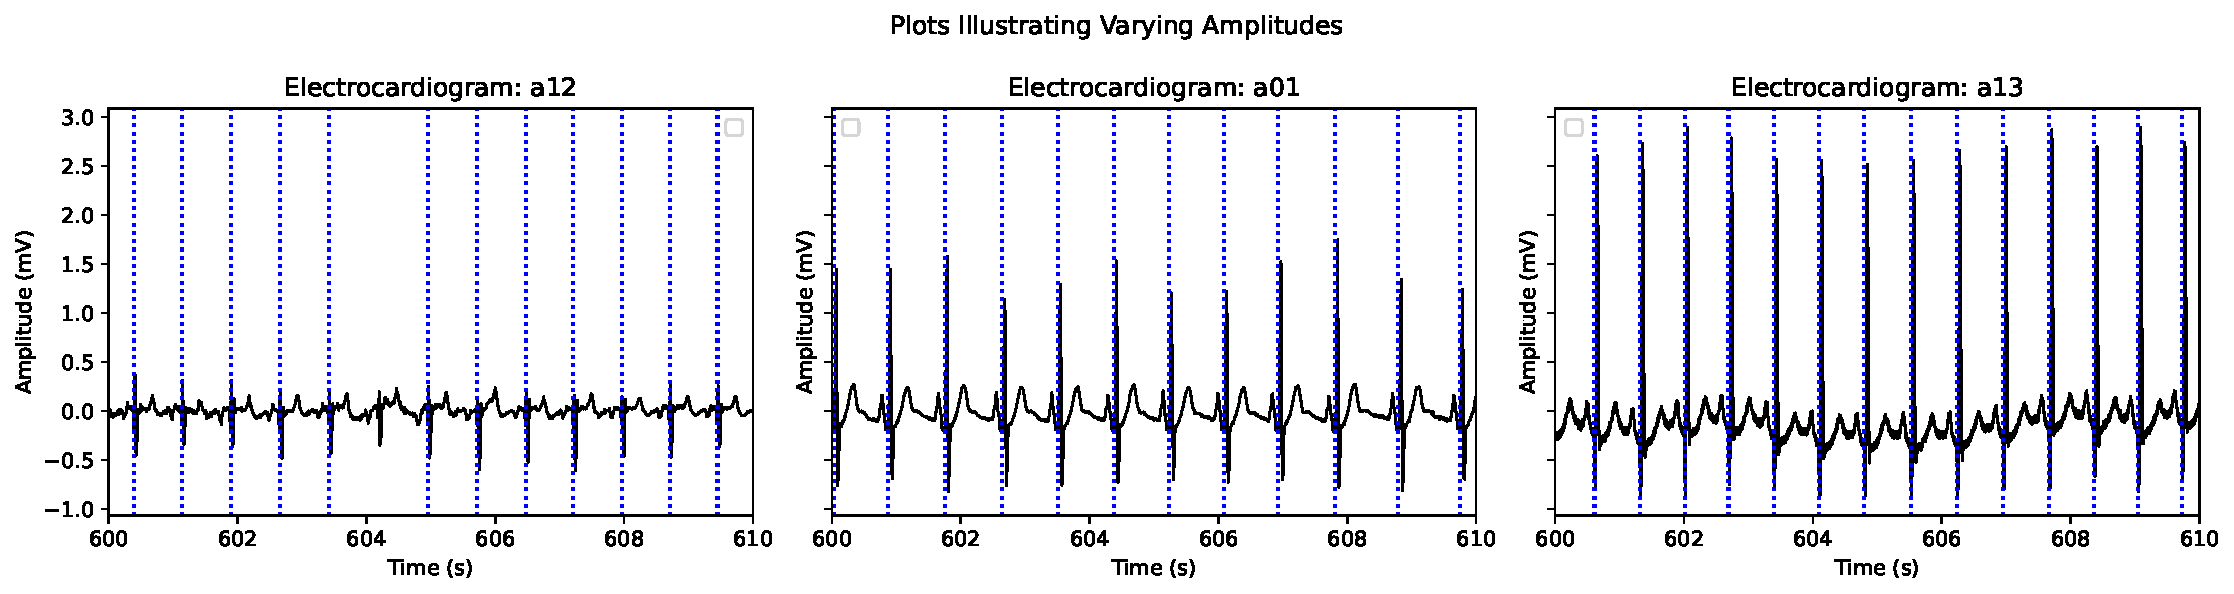
\includegraphics[width=\textwidth]{figures/Vary_amp_ECG.pdf}
    \caption{ECG datasets illustrating differing amplitude magnitudes.}
    \label{fig:ecg-amp-signal}
\end{figure}
\begin{figure}[H]
    \centering
    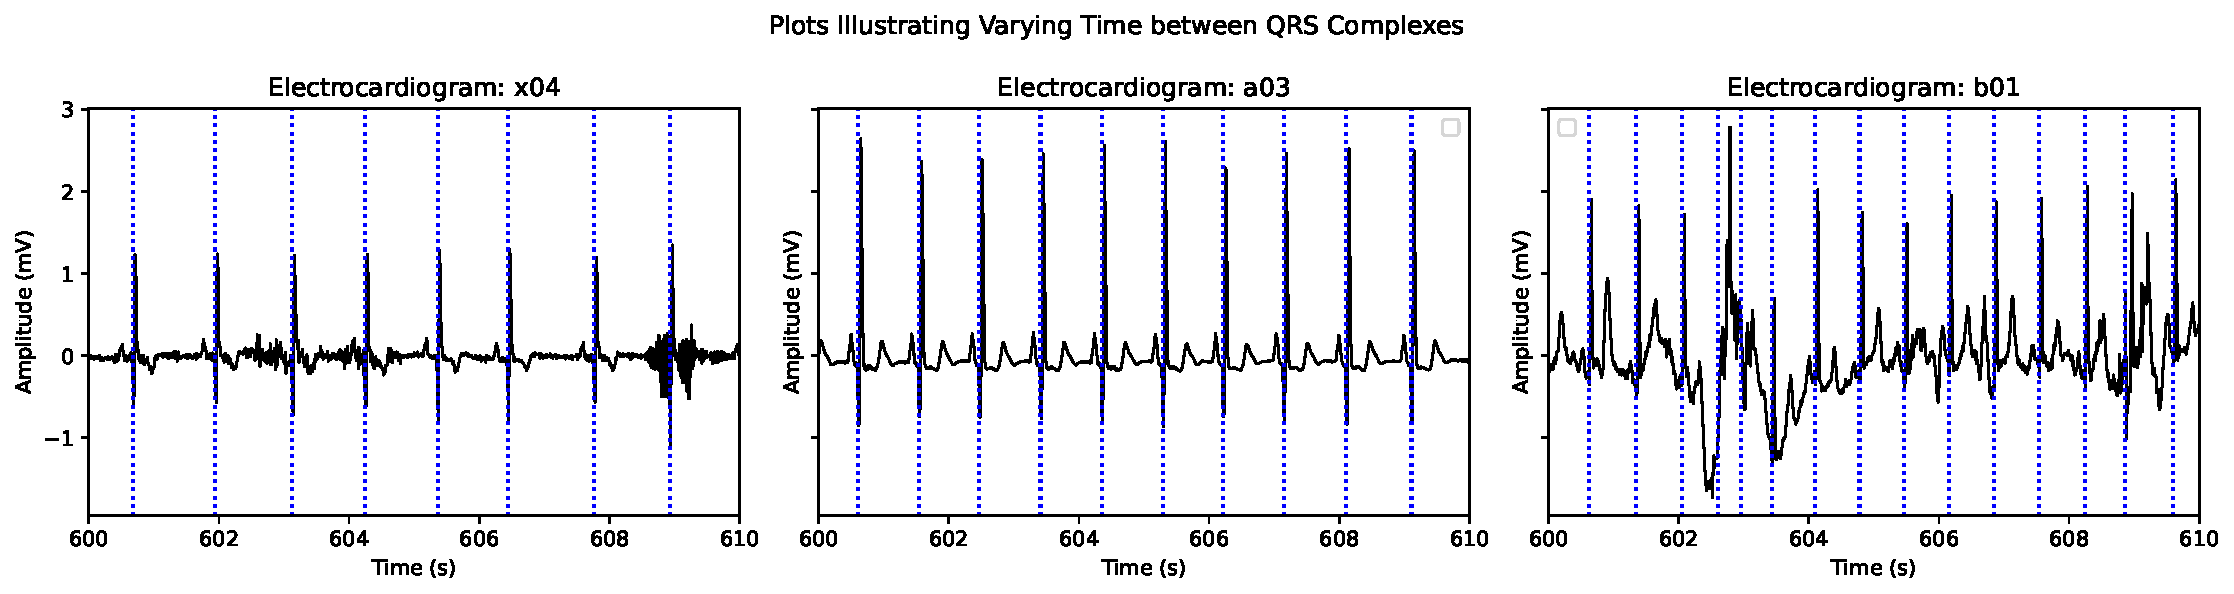
\includegraphics[width=\textwidth]{figures/Vary_time_ECG.pdf}
    \caption{ECG datasets illustrating differing time intervals between QRS 
    Complexes.}
    \label{fig:ecg-time-signal}
\end{figure}
\begin{figure}[H]
    \centering
    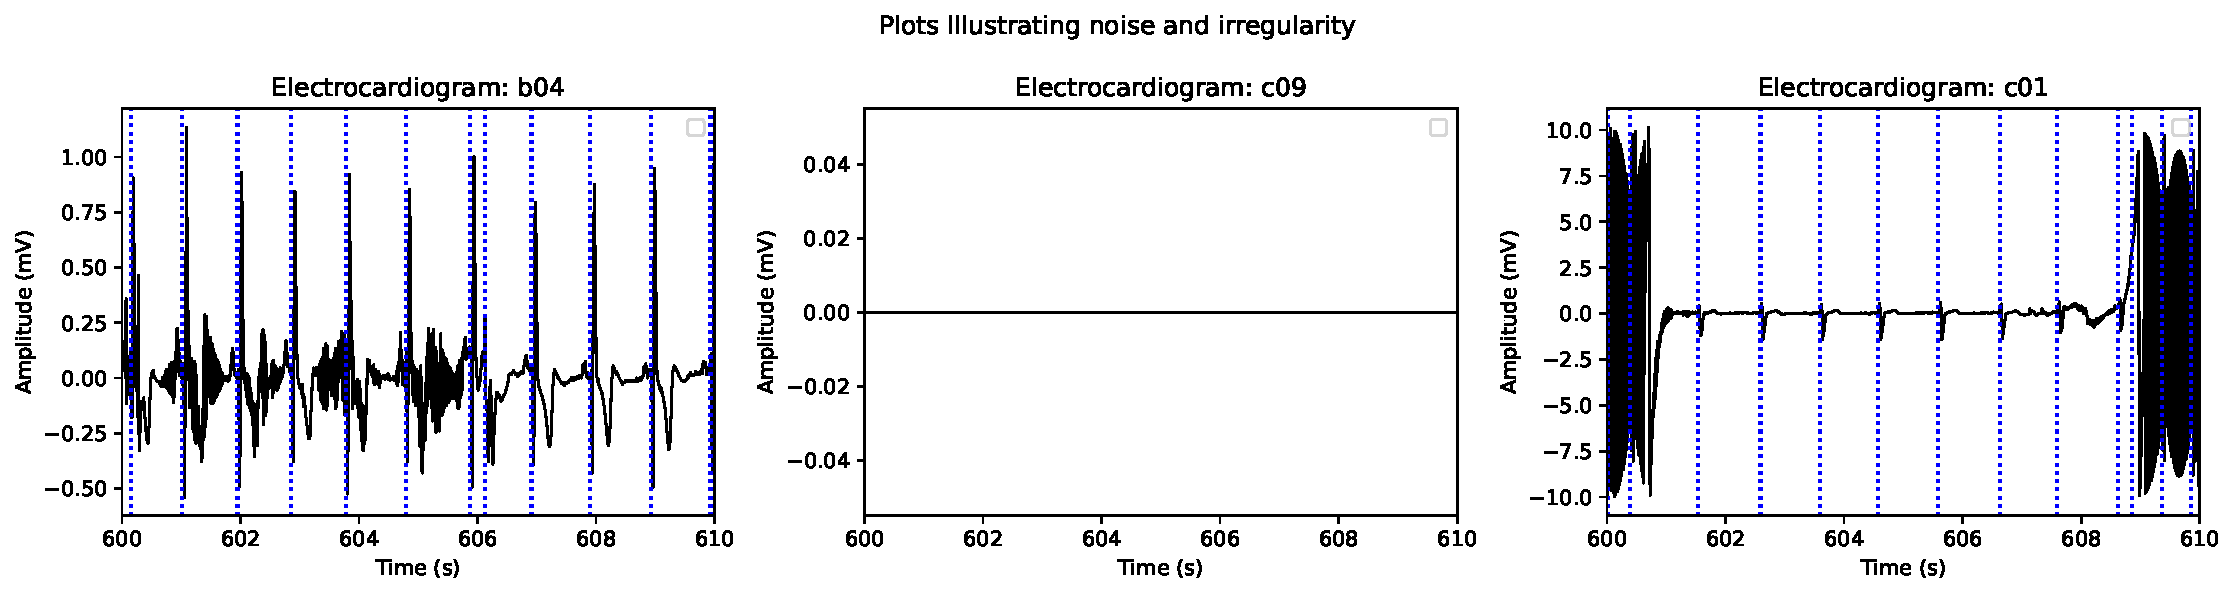
\includegraphics[width=\textwidth]{figures/noise_ECG.pdf}
    \caption{ECG datasets illustrating the existence of noise and artifacts in the data.}
    \label{fig:ecg-noise-signal}
\end{figure}
Figure~\ref{fig:ecg-amp-signal} shows how the amplitude of the QRS signal can vary signficantly across datasets, Figure~\ref{fig:ecg-time-signal} illustrates
that the time between QRS complexes also varies, and Figure~\ref{fig:ecg-noise-signal} highlights the existence of noise and artifacts in some datasets. 
Further, we can also see in the following (Figure \ref{fig:ecg-amp-single-signal}) that within a data set the QRS complex amplitude can be only slightly
larger than the amplitude of other peaks in the data. 
\begin{figure}[H]
    \centering
    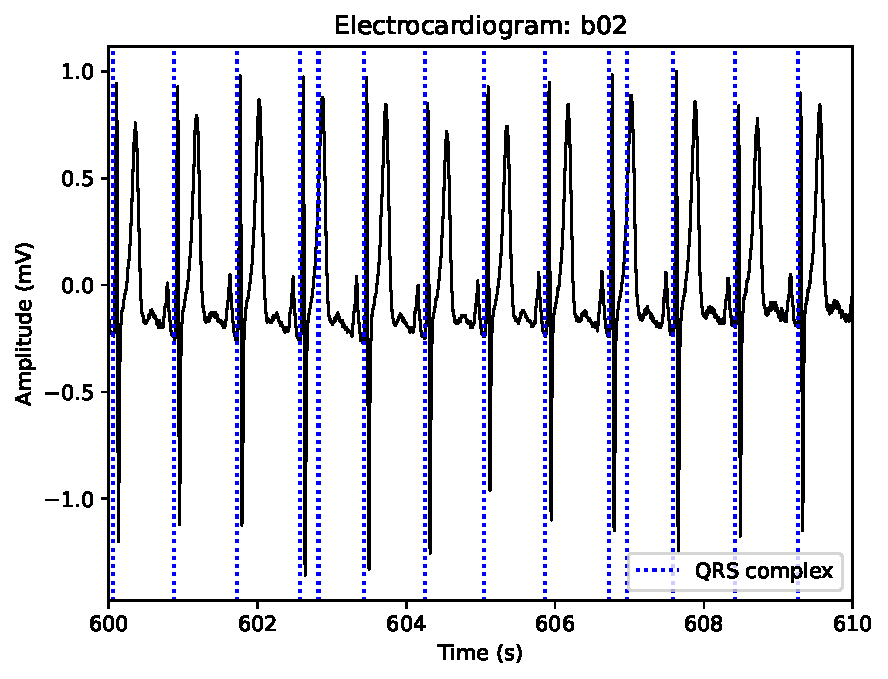
\includegraphics[width=0.50\textwidth]{figures/Close_amp_ECG.pdf}
    \caption{ECG signal illustrating QRS amplitude can be close to other peak
    amplitudes.}
    \label{fig:ecg-amp-single-signal}
\end{figure}


Going forward we focus on testing our algorithms against these data 
samples: a01, a12, a13, a03, x04, b01, b02, c02, as they represent 
how amplitude of QRS complexes, and the time between can vary. This is important as those 
characteristics will form the basis of our Respiratory Rate estimation and we need to ensure that 
the RR peak identifcation algorithm is robust against variation in these traits. 






